\documentclass[a4paper,12pt]{article}
\usepackage[a4paper,top=1.3cm,bottom=2cm,left=1.5cm,right=1.5cm,marginparwidth=0.75cm]{geometry}
\usepackage{cmap}
\usepackage{mathtext}
\usepackage[T2A]{fontenc}
\usepackage[utf8]{inputenc}
\usepackage[english,russian]{babel}
\usepackage{siunitx}

\usepackage{graphicx}

\usepackage{wrapfig}
\usepackage{tabularx}
\usepackage{multirow}

\usepackage{hyperref}
\usepackage[rgb]{xcolor}
\hypersetup{
colorlinks=true,urlcolor=blue
}
\usepackage{amsmath,amsfonts,amssymb,amsthm,mathtools}
\usepackage{icomma}
\mathtoolsset{showonlyrefs=false}
\usepackage{euscript}
\usepackage{mathrsfs}
\DeclareMathOperator{\sgn}{\mathop{sgn}}
\newcommand*{\hm}[1]{#1\nobreak\discretionary{}
{\hbox{$\mathsurround=0pt #1$}}{}}

%%% Заголовок
\author{Макаров Лев Евгеньевич}
\title{Лабораторная работа №3.3.4

Эффект Холла в полупроводниках
}
\date{\today}

\begin{document}

\begin{titlepage}
	\begin{center}
		{\large МОСКОВСКИЙ ФИЗИКО-ТЕХНИЧЕСКИЙ ИНСТИТУТ (НАЦИОНАЛЬНЫЙ ИССЛЕДОВАТЕЛЬСКИЙ УНИВЕРСИТЕТ)}
	\end{center}
	\begin{center}
		{\large Физтех-школа фотоники, электроники и молекулярной физики}
	\end{center}
	
	
	\vspace{4.5cm}
	{\huge
		\begin{center}
			{\bf Отчёт о выполнении лабораторной работы 3.3.4}\\
			Эффект Холла в полупроводниках
		\end{center}
	}
	\vspace{2cm}
	\begin{flushright}
		{\LARGE Автор:\\ Макаров Лев Евгеньевич \\
			\vspace{0.2cm}
			Б04-306}
	\end{flushright}
	\vspace{8cm}
	\begin{center}
		Долгопрудный 2024
	\end{center}
\end{titlepage}

\section{Введение}

\textbf{Цель работы:} 
\begin{enumerate}
	\item измерение подвижности и концентрации носителей заряда в полупроводниках
\end{enumerate}

\textbf{В работе используются:} 
\begin{itemize}
    \item электромагнит с регулируемым источником питания
    \item вольтметр
    \item амперметр
    \item милливольтметр
    \item милливеберметр
    \item генератор
    \item образцы легированного германия
\end{itemize}
\medskip

\section{Теоретические сведения}

\textbf{Корректность измерения напряжения.} Исключить падение напряжения, вызванного неточностью положений контактов 3 и 4 (если они не на одной эквипотенциали) можно с помощью изменения направления магнитного поля, пронизывающего образец. Поскольку если повернуть поле, ЭДС Холла поменяет знак, но по модулю не изменится, ЭДС Холла можно получить следующим образом:
\begin{equation*}
    U_\perp = \frac{1}{2} (U_{34}^{(+)} - U_{34}^{(-)}),
\end{equation*}
где $U_{34}^{(\pm)}$ -- показание вольтметра, полученное при одном из противоположных направлений магнитного поля в зазоре.

Иной метод: при каждом значении тока через образец измерять напряжение между точками 3 и 4 в отсутствие магнитного поля. Если ток через образец не меняется, то это дополнительное напряжение $U_0$ также не меняется. Тогда:
\begin{equation*}
    U_\perp = U_{34} - U_0.
\end{equation*}

\textbf{Характер проводимости.} По знаку $U_\perp$ можно определить характер проводимости -- \textit{электронный} или \textit{дырочный}. Для этого необходимо знать направление тока в образце и направление магнитного поля.

Измерив ток $I$ в образце и напряжение $U_{35}$ между контактами 3 и 5 в отсутствие магнитного поля, можно, зная параметры образца, рассчитать проводимость материала образца по формуле:
\begin{equation*}
    \rho_0 = \frac{al}{L_{35}}\cdot\frac{U_{35}}{I},
\end{equation*}
где $L_{35}$ -- расстояние между контактами 3 и 5, $l$ -- ширина образца, $a$ -- его толщина.

\section{Эксперементальная установка}

Электрическая схема установки для измерения ЭДС Холла представлена на рис. \ref{ust}. В зазоре электромагнита (рис. 1а) создаётся постоянное магнитное поле, величину которого можно менять с помощью регулятора источника питания электромагнита. Ток питания электромагнита измеряется амперметром А1 (внешним или встроенным в источник). Направление тока в обмотках электромагнита меняется переключением разъёма К1. Градуировка электромагнита (связь тока с индукцией поля) проводится при помощи милливеберметра или миллитесламетра на основе датчика Холла. 

Прямоугольный образец из легированного германия, смонтированный в специальном держателе (рис. 1б, рис. \ref{Sample}), подключается к источнику питания ($\simeq$ 1,5 В). При замыкании ключа $К_2$ вдоль длинной стороны образца течёт ток, величина которого регулируется реостатом $R_2$ и измеряется миллиамперметром $А_2$.

В образце, помещённом в зазор электромагнита, между контактами 3 и 4 возникает разность потенциалов $U_{34}$, которая измеряется с помощью вольтметра V.

\begin{figure}[!h]
    \center
    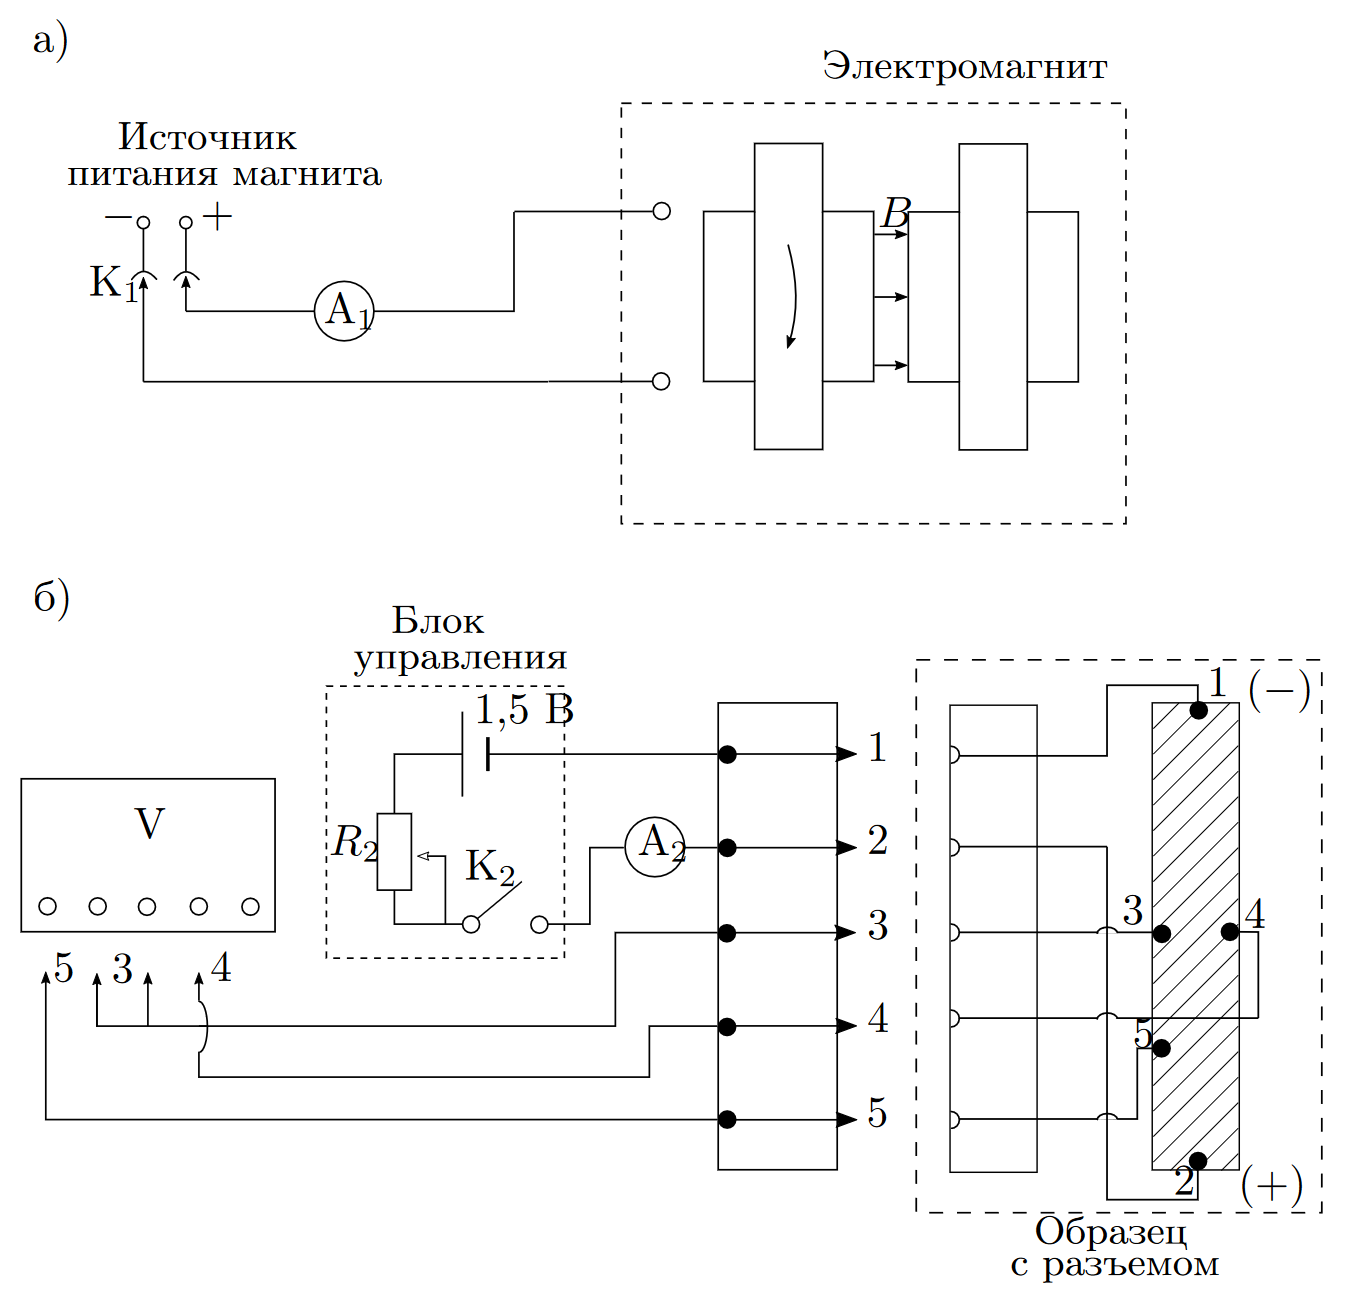
\includegraphics[scale=0.6]{ust.png}
    \caption{Схема установки для исследования вынужденных колебаний}
    \label{ust}
\end{figure}


\section{Результаты измерений и обработка данных}

\subsection{Подготовка приборов}

Включим милливольтметр и подождем пока закончиться его автонастройка. Подключим к нему провода 3-4.

\subsection{Проверка образца}

Проверим ток через образец, Необходимо убедиться, что ток реостатом можно изменять от 0 до 1 мА.

\subsection{Регулировка электромагнита}

Измерим предел изменения тока через электромагнит $I_M^{max}$.

\begin{equation*}
    I_M^{max} = 1,62 \ \text{А}
\end{equation*}

Поэтому при змерениях будем поднимать ток $I_M$ не более, чем до 1,5 А.

\subsection{Измерение калибровочной кривой}

Измерим зависимость индукции магнитного поля B в зазоре электромагнита в зазоре от тока $I_M$.
Снимем показания милливеберметра для нескольких значений тока $I_M$ и поместим в таблицу \ref{table:1}.

Значение $SN = (75,0 \pm 0,5) \ \text{см}^2 \text{вит}$ 

\begin{table}[!ht]
    \centering
    \begin{tabular}{|l|l|l|l|}
    \hline
        N & $I_M$, A & $\Phi$, мВб & $B$, Тл \\ \hline
        1 & 0,19 & 1,4 & 0,19 \\ \hline
        2 & 0,37 & 2,7 & 0,36 \\ \hline
        3 & 0,56 & 4,1 & 0,55 \\ \hline
        4 & 0,75 & 5,5 & 0,73 \\ \hline
        5 & 0,93 & 6,6 & 0,88 \\ \hline
        6 & 1,13 & 7,5 & 1,00 \\ \hline
        7 & 1,30 & 8,2 & 1,09 \\ \hline
        8 & 1,50 & 8,7 & 1,16 \\ \hline
    \end{tabular}\caption{\textit{Зависимость индукции магнитного поля $B$ от тока $I_M$}}\label{table:1}
\end{table}

Погрешность измерения тока $I_M$ равна $\sigma_M = 0,03$ А. Погрешность измерения индукции поля $\sigma_\Phi = 0.2$ мВб, так как измеряется как дельта между начальным и конечным. Посчитаем индукцию через катушку из формулы $\Phi = B SN$ и запишем в таблицу \ref{table:1}.

Погрешность измерения $B$ можно вычислить по формуле:

\begin{equation}
    \sigma_B = B \sqrt{\left( \frac{\sigma_\Phi}{\Phi} \right)^2 + \left( \frac{\sigma_{SN}}{SN} \right)^2} \approx 0,03 \ \text{Тл}
\end{equation}

Погрешность $\sigma_B$ получилась одинаковой для всех измерений.

\subsection{Определение $U_0$}

Вствавим образец в зазор электромагнита и имзерим $U_0 = 0,264$ мв при токе $I = (0,37 \pm 0,03)$ мА. Это значение будет меняться при изменении тока.

\subsection{Измерение ЭДС Холла}
\label{punkt:4.6}

Замерим напряжение $U_{34}$ при постоянном токе $I$ при разных значениях $I_M$ и результаты измерений запишем в таблицу \ref{table:2}. Погрешность измерения $U_{34}$ составляет $\sigma_{34} = 0,01$ мВ.

\begin{table}[!ht]
    \centering
    \begin{tabular}{|l|l|l|}
    \hline
        $N$ & $I_M$, A & $U_{34}$, мВ \\ \hline
        1 & 0,26 & 1,27 \\ \hline
        2 & 0,50 & 2,44 \\ \hline
        3 & 0,75 & 3,61 \\ \hline
        4 & 1,00 & 4,60 \\ \hline
        5 & 1,25 & 5,21 \\ \hline
        6 & 1,50 & 5,62 \\ \hline
    \end{tabular}\caption{\textit{Зависимость напряжения $U_{34}$ от тока $I_M$ при токе $I = 0,37$ мА}}\label{table:2}
\end{table}

\subsection{Измерения при других значениях $I$}

Повторим результаты измерений пункта \ref{punkt:4.6} для других значений тока $I$ до 1 мА и результаты измерений запишем в таблицу \ref{table:3}.

\begin{table}[!ht]
    \centering
    \begin{tabular}{|l|l|l|l|l|l|l|l|l|}
    \hline
        ~ & $I$, мA & 0,46 & 0,55 & 0,64 & 0,73 & 0,82 & 0,91 & 1,00 \\ \hline
        $N$ & $I_M$, A & $U_{34}$, мВ & $U_{34}$, мВ & $U_{34}$, мВ & $U_{34}$, мВ & $U_{34}$, мВ & $U_{34}$, мВ & $U_{34}$, мВ \\ \hline
        1 & 0,25 & 1,49 & 1,76 & 2,12 & 2,37 & 2,63 & 2,88 & 3,22 \\ \hline
        2 & 0,50 & 3,04 & 3,60 & 4,25 & 4,87 & 5,35 & 5,99 & 6,61 \\ \hline
        3 & 0,75 & 4,44 & 5,31 & 6,19 & 7,04 & 7,85 & 8,77 & 9,68 \\ \hline
        4 & 1,00 & 5,65 & 6,68 & 7,82 & 8,87 & 9,98 & 11,07 & 12,19 \\ \hline
        5 & 1,25 & 6,41 & 7,61 & 8,86 & 10,11 & 11,35 & 12,58 & 13,83 \\ \hline
        6 & 1,50 & 6,92 & 8,22 & 9,58 & 10,92 & 12,26 & 13,61 & 14,95 \\ \hline
    \end{tabular}\caption{\textit{Зависимость напряжения $U_{34}$ от тока $I_M$}}\label{table:3}
\end{table}

\subsection{Измерения в обратном направлении}

Проведем аналогичные измерения при обратном направлении магнитного поля и результаты запишем в таблицу \ref{table:4}.

\begin{table}[!ht]
    \centering
    \begin{tabular}{|l|l|l|}
    \hline
        $N$ & $I_M$, A & $U_{34}$, мВ \\ \hline
        1 & 0,26 & -3,07 \\ \hline
        2 & 0,50 & -6,44 \\ \hline
        3 & 0,75 & -9,37 \\ \hline
        4 & 1,00 & -11,79 \\ \hline
        5 & 1,25 & -13,41 \\ \hline
        6 & 1,50 & -14,14 \\ \hline
    \end{tabular}\caption{\textit{Зависимость напряжения $U_{34}$ от тока $I_M$ при обратном направлении магнитного поля}}\label{table:4}
\end{table}

\subsection{Определение знака заряда носителей}

На клемме 4 скапливается отрицательный заряд, следовательно, с учетом направления тока и магнитного поля. Носителями заряды выступают отрицательно заряженные частицы. То есть электронный способ проводимости.

\subsection{Измерение удельной проводимости}

Удалим держатель с образцом из зазора. Установим ток через образец $I = 1$ мА. Подключим клеммы 3-5 и измерим напряжение между ними $U_{35} = (85,35 \pm 0,01)$ мВ.

\subsection{Характеристики приборов}

Запишем зарактеристики приборов:

\begin{equation*}
    l = (15,0 \pm 0,5) \ \text{мм}
\end{equation*}
\begin{equation*}
    h = (2,0 \pm 0,5) \ \text{мм}
\end{equation*}
\begin{equation*}
    a = (8,0 \pm 0,5) \ \text{мм}
\end{equation*}

\subsection{Калибровочный график}

Построим график зависимости $B(I_M)$. Для этого аппроксимируем наилучшую прямую МНК. график изобразим на рисунке \ref{graph:1}.


\begin{equation}\label{eq:mnk}
    k = (0,76 \pm 0,04) \ \text{Тл}/\text{А},
    \ \text{а} \ \  b = (0,10 \pm 0,02) \ \text{Тл}
\end{equation}

\subsection{Вычисление ЭДС Холла}

Построим график зависимости ЭДС Холла от индукции $B$ при нескольких значениях тока $I$. $B$ получим экстраполируя по результатам прошлого пункта. График нанесем на рисунок \ref{graph:2}.

\subsection{Определение постоянной Холла}

Построим график зависимости коэффициентов $k$ от тока $I$. График нанесем на рисунок \ref{graph:3}.

\begin{equation}\label{eq:mnk}
    \gamma = (12,93 \pm 0,03) \ \text{В}/\text{Тл} / \text{мА}
\end{equation}

Из формулы (3.27) следует, что

\begin{equation*}
    R_H = h \frac{dU / dB}{I} = h \frac{k}{I} = h \gamma = 2 \cdot 12,93 \approx (25 \pm 7) \ \frac{\text{м}^3}{\text{Кл}}
\end{equation*}

\subsection{Рассчет параметров проводимости}

Удельную проводимость и удельное сопротивление можно получить из формулы:

\begin{equation*}
    R_H = \frac{1}{nq} \implies n = \frac{1}{R_H q} \approx (2,4 \pm 0,6) \cdot 10^{-17} \ \text{м}^{-3}
\end{equation*}
\begin{equation*}
    \sigma_0 = \frac{I l}{U_{35} ha} = \frac{1 \cdot 10^{-3} \cdot 15 \cdot 10^{-3}}{85,35 \cdot 10^{-3} \cdot 2 \cdot 10^{-3} \cdot 8 \cdot 10^{-3}} \approx (11 \pm 3) \ \left( \text{Ом} \cdot \text{м} \right)^{-1}
\end{equation*}

Вычислим удельное сопротивление

\begin{equation*}
    \rho_0 = \frac{1}{\sigma_0} \approx (0,09 \pm 0,02) \ \text{Ом} \cdot \text{м}
\end{equation*}

\subsection{Вычисление подвижности}

Подвижность заряда вычисляется:

\begin{equation*}
    \mu = \frac{\sigma_0}{en} \approx (2,8 \pm 0,7) \cdot 10^{40} \ \frac{\text{см}^2}{\text{В} \cdot \text{с}} 
\end{equation*}

\subsection{Другие графики зависимости}

Во время работы был исследован эффект Холла в полупроводниках. Результаты на несколько порядков не сходятся с табличными значениями. 

Возможно это обЪясняется наличием примесей в образце.


\begin{figure}[h!]
        \centering
	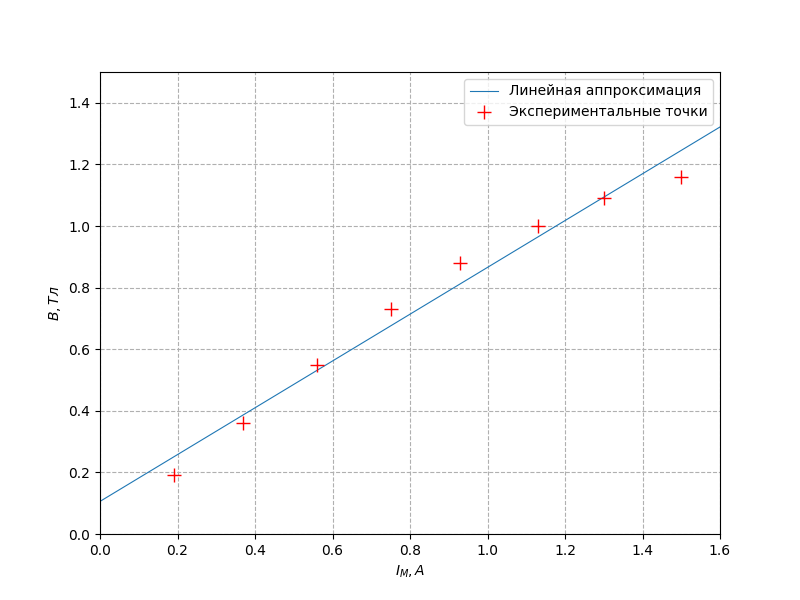
\includegraphics[width=1.1\textwidth]{graph-I_M-B.png}
	\caption{\textit{График зависимости $B$ от $I_M$}}
	\label{graph:1}
\end{figure}

\begin{figure}[h!]
        \centering
	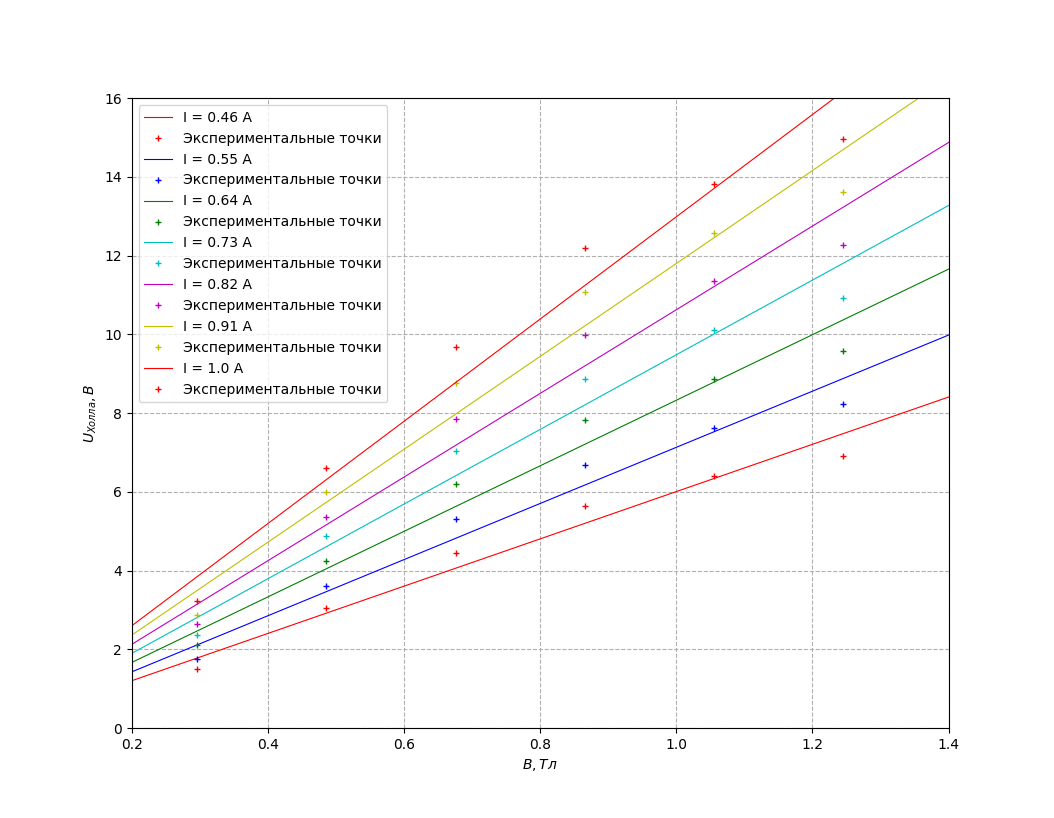
\includegraphics[width=1.1\textwidth]{graph-B-U_34.png}
	\caption{\textit{График зависимости $U_{34}$ от $B$}}
	\label{graph:2}
\end{figure}

\begin{figure}[h!]
        \centering
	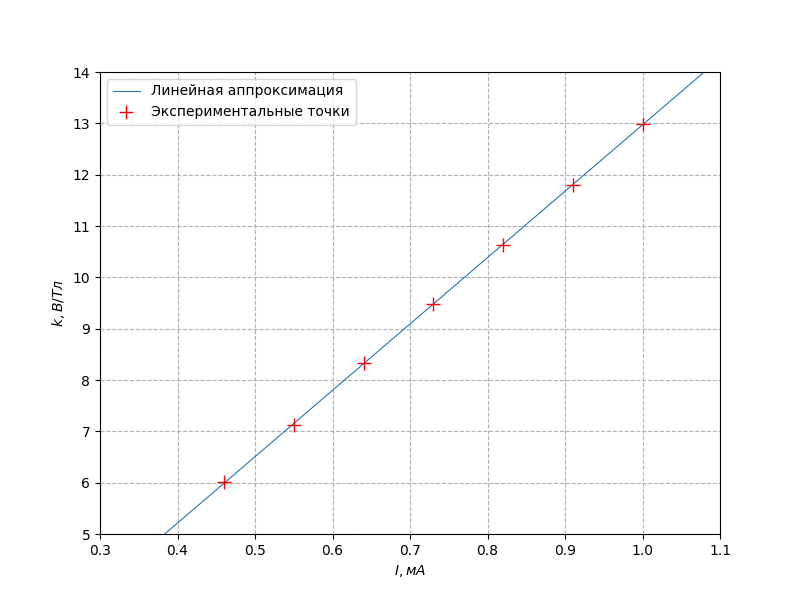
\includegraphics[width=1.1\textwidth]{graph-I-k.png}
	\caption{\textit{График зависимости $k$ от $I$}}
	\label{graph:3}
\end{figure}

\end{document}